\documentclass{article}
\usepackage[utf8]{inputenc}
\usepackage{amsfonts}
\usepackage{amsmath}
\renewcommand{\labelitemii}{$\circ$}
%% Custom commands
\newcommand{\E}[1]{\langle #1 \rangle} % shortcut for expectation
\newcommand{\norm}[3]{\mathcal{N}\left(#1; #2, #3\right)} %shorcut normal distributions

\usepackage[final]{graphicx}
\graphicspath{ {./images/} }

%% make sections floats barries
\usepackage{placeins}

\let\Oldsection\section
\renewcommand{\section}{\FloatBarrier\Oldsection}

\let\Oldsubsection\subsection
\renewcommand{\subsection}{\FloatBarrier\Oldsubsection}

\let\Oldsubsubsection\subsubsection
\renewcommand{\subsubsection}{\FloatBarrier\Oldsubsubsection}

%%% hyperlinks into document
% see https://www.overleaf.com/learn/latex/Hyperlinks
\usepackage{hyperref}
\hypersetup{
    colorlinks=true,
    linkcolor=black,
    filecolor=magenta,      
    urlcolor=cyan,
    pdftitle={Master Thesis}
    }
    
%%% removeparagraph indent
\parindent=0pt

%%% === add support \subsubparagraph and \sssparagraph
% see https://tex.stackexchange.com/questions/94402/creating-a-subsubparagraph
\makeatletter
\newcounter{subsubparagraph}[subparagraph]
\renewcommand\thesubsubparagraph{%
  \thesubparagraph.\@arabic\c@subsubparagraph}
\newcommand\subsubparagraph{%
  \@startsection{subsubparagraph}    % counter
    {6}                              % level
    {\parindent}                     % indent
    {3.25ex \@plus 1ex \@minus .2ex} % beforeskip
    {-1em}                           % afterskip
    {\normalfont\normalsize\itshape\bfseries}}
\newcommand\l@subsubparagraph{\@dottedtocline{6}{10em}{5em}}
\newcommand{\subsubparagraphmark}[1]{}
\def\toclevel@subsubparagraph{6}
\makeatother
% ---
\makeatletter
\newcounter{sssparagraph}[sssparagraph]
\renewcommand\thesssparagraph{%
  \thesubsubparagraph.\@arabic\c@sssparagraph}
\newcommand\sssparagraph{%
  \@startsection{sssparagraph}    % counter
    {7}                              % level
    {\parindent}                     % indent
    {3.25ex \@plus 1ex \@minus .2ex} % beforeskip
    {-1em}                           % afterskip
    {\normalfont\normalsize\itshape}}
\newcommand\l@sssparagraph{\@dottedtocline{7}{10em}{5em}}
\newcommand{\sssparagraphmark}[1]{}
\def\toclevel@sssparagraph{6}
\makeatother

%%% ===

\usepackage{listings}

\usepackage{biblatex}
\addbibresource{Thesis-references.bib}

\title{Master Thesis. Imputation of Eddy Covariance meteorological time series using Kalman filters}
\author{Simone Massaro}
\date{January 2023}

\begin{document}

\maketitle
\tableofcontents
\clearpage

\section{Introduction}

\subsection{Eddy Covariance and meteo}

Eddy Covariance is a state of the art technique for measuring fluxes exchanges between ecosystems and the atmosphere [Uubinet, M., Vesala, T.  Papale, D. (Eds.). Eddy Covariance: A Practical Guide to Measurement and Data Analysis (Springer Netherlands, Dordrecht, 2012)].  The technique allows fluxes measurements at a high temporal resolution and ecosystem level. The use of Eddy Covariance data is key is many ecology research [TODO cite].
The core of standard Eddy Covariance tower is the 3D anemometer and gas analyzers, which allows to estimated the fluxes of interests ($CO_2$, $H_20$). However those are not the only variable measured, as many additional on-site measurements are needed for   [TODO cite something like ICOS]

\begin{itemize}
    \item what is Eddy Covariance
    \item use of EC data
    \item how EC measures fluxes: anemometer + gas analyser
    \item other measurements: meteo, ecology
\end{itemize}

\begin{itemize}
\item why there are gaps [cite]
\end{itemize}


\subsection{Why need to do meteo gap filling in EC}

\begin{itemize}
    \item ecological modelling that use EC data for validations (eg \cite{kramer_evaluation_2002}) they need a complete input, and the meteo data needs to from the site
    \item meteo are used as drivers for Fluxes gap filling 
    \item long term averages
\end{itemize}

\paragraph{How to fill gaps}

\begin{itemize}
    \item analyze time series
    \item variable correlation
    \item use other measurements
\end{itemize}


\subsection{Current approaches}

\begin{itemize}
\item Gap filling part of EC pipelines
\item OneFlux is the reference fluxes post processing pipeline
\item it implements two types of gap filling: MDS and ERA
\end{itemize}
\paragraph{Marginal Distribution Sampling (MDS)}
\begin{itemize}
        \item 
    \end{itemize}

\paragraph{ERA-Interim}

\paragraph{Other approaches}
\begin{itemize}
\item OneFlux is not the only processing pipeline
\item other libraries implement same method (eg. REddyProc, [others?])
\item DINGO from OzFlux different as use measurements from local other meteo station (\cite{beringer_technical_2017}) . 
\item However, it uses data from the Australian meteo service,
\item cannot be easily used worldwide
\end{itemize}

\subsection{Limitation current approach}
\begin{itemize}
\item the current approach is limited
\item doesn't combine imputation approaches
\item is not good especially for short/medium gaps
\item focus of community is on fluxes, since there are a lot of gaps in fluxes
\item different methods used (ANN, [more citation])
\item relative low importance of meteo due to lower amount of gaps
\item can do better for meteo than state of art
\item there is  ERA , actually now there is also ERA-5 Land which has a much higher resolution
\item small amount of gaps
\end{itemize}

\subsection{Uncertainty of imputation}
\begin{itemize}
\item current system have a quality flag, but is very limited as it has only tow possible values (1 or 2) and depends on an arbitrary limit on window gap len
\item doesn't depend on conditions
\item can build a model that predict an uncertainty for every time point
\item successful in other context [citeeeeeee]
\item downstream user don't use uncertainty now, because is not available
\item but believe there is potential for it [citeeeeee]
\end{itemize}

\subsection{Kalman Filters}
\begin{itemize}
\item need to find a modelling approach that can meet those requirements
\item combine 3 gap filling approaches
\item provide uncertanties
\item by analyzing the gap length in Fluxnet for meteo variables the gaps are short (see Appendix )
\item there are many possible approaches (eg. GP-VAE, random forests)
\item so we likely don't need a very complex model
\item kalman filter is on of the simplest model that can fit the requirements
\end{itemize}


\subsection{Research question}
\begin{itemize}
\item develop a meteo EC imputation method using Kalman Filters
\item assess the performance of the method
\item compare with the state of the art
\end{itemize}


\section{Methods}

\subsection{Kalman Filter Theory}

\subsubsection{Probabilistic Machine Learning}

\begin{itemize}
\item probability
\item Conditional probability
\item Bayes theorem
\item Gaussian Inference
\end{itemize}

\subsubsection{Notation}

[figure:; table with variable names and visualization of gap]

\begin{itemize}
\item $t$  Number of time steps
\item observations
\begin{itemize}
    \item $n$  Number of variables observed
    \item $y_{:,t}$ or $y_t$ vector of all the $n$ variables at time $t$, $\in \mathbb{R}^n $
    \item $y_{n,:}$ vector of the $n$th variable at for time steps in $t$, $\in \mathbb{R}^T$
    \item $y_{n,t}$ $n$th variable at time $t$, $\in \mathbb{R}$ 
    \item $Y_M = [x_{:,1}, ... x_{:, t}]$ Matrix with all the $n$ variables at all time steps, $\in \mathbb{R}^{n \times t}$ 
    \item $Y$ is a vector obtained by "flattening" $X_M$, by putting next to each other all variable at time $t$, $\in \mathbb{R}^{(n \cdot t)}$
    \item $y^{ng}_t$ vector of variable that are not missing (ng = not gap)) at time $t$, $\in \mathbb{R}^{n_{ng}}$. Note at different times the shape of this vector can change
    \item $Y^{ng}$ all observations
\end{itemize}

\item Latent state
\begin{itemize}
    \item $k$  Number of variables in latent state
    \item $x_{:,t}$ or $x_t$ vector of all the $k$ state variables at time $t$, $\in \mathbb{R}^k $
    \item $x_{k,:}$ vector of the $k$th variable at for time steps in $t$, $\in \mathbb{R}^t$
    \item $x_{k,t}$ $k$th variable at time $t$, $\in \mathbb{R}$ 
    \item $X_M = [x_{:,1}, ... x_{:, t}]$ Matrix with all the $k$ variables at all time steps, $\in \mathbb{R}^{k \times t}$ 
    \item $X$ is a vector obtained by "flattening" $X_M$, by putting next to each other all variable at time $t$, $\in \mathbb{R}^{(k \cdot t)}$
\end{itemize}

\end{itemize}


\subsubsection{Basics Kalman Filter}

\begin{itemize}
    \item why Kalman filter
    \item picture of Kalman filter state
\end{itemize}

\paragraph{Description}

The latent state ($x$) is modelled using a Markov chain. Which means that the state at time $t$ depends only on the state at time $t-1$ and not the states at previous times

\paragraph{Assumptions}

\begin{equation}\label{state_eq}
p(x_t | x_{t-1}) = \mathcal{N}(Ax_{t-1} + b, Q)
\end{equation}

The observation are derived from the state using a linear map plus random noise

\begin{equation}\label{obs_from_state}
    p(y_t | x_t) = \mathcal{N}(Hx_t + d, R)
\end{equation}


\subsubsection{Time update}

The probability distribution of state at time $t$ is computed using the state a time $t-1$

The state at time $t-1$ has a distribution $$ p(x_{t-1}) = \mathcal{N}(m_{t-1}, P_{t-1}) $$ 

Combining this equation with equation \ref{state_eq} and using the properties of a linear map of a Gaussian distribution we obtain:

\begin{equation}
    \label{filter_predict}p(x_t) = \mathcal{N}(x_t; m_t^-, P_t^-)
\end{equation} 

where:
\begin{itemize}
    \item predicted state mean: $m_t^- = Am_{t-1} + B c_t + d$   
    \item predicted state covariance: $P_t^- = AP_{t-1}A^T + Q$
\end{itemize}

The mean and the covariance of the state at time $0$ are parameters of the models that are learned

\subsubsection{Measurement update}

The probability distribution of state at time $t$ is corrected using the observations at time $t$

This uses equation \ref{obs_from_state} and the formula for posterior distributions for Gaussian distributions.

\begin{equation}\label{filter_update}
 p(x_t|y_t) = \mathcal{N}(x_t; m_t, P_t)   
\end{equation}
    
where:

\begin{itemize}
    \item predicted obs mean: $z_t = Hm_t^- + d$   
    \item predicted obs covariance: $S_t = HP_t^-H^T + R$
    \item Kalman gain $K_t = P_t^-H^TS_t^{-1}$ 
    \item corrected state mean: $m_t = m_t^- + K_t(y_t - z_t)$ 
    \item corrected state covariance: $P_t = (I-K_tH)P_t^-$ 
\end{itemize}

\paragraph{Missing observations}
If all the observations at time $t$ are missing the correct step is skipped and the filtered state at time $t$ (equation \ref{filter_correct}) is the same of the filtered state.

If only some observations are missing a variation of equation \ref{filter_correct} can be used.

$y^{ng}_t$ is a vector containing the observations that are not missing at time $t$. 

It can be expressed as a linear transformation of $y_t$

$$ y^{ng}_t = My_t$$

where $M$ is a mask matrix that is used to select the subset of $y_t$ that is observed. $M \in \mathbb{R}^{n_{ng} \times n}$ and is made of rows which are made of all zeros but for an entry 1 at column corresponding to the of the index non-missing observation.

For example, if $y_t = [y_{0,t}, y_{1,t}, y_{2,t}]^T$ and $y_{0,t}$ is the missing observation then

$$ M = \left[\begin{array}{ccc}
    0 & 1 & 0 \\
    0 & 0 & 1
\end{array}\right]$$
hence:

$$ p(y^{ng}_t) = \mathcal{N}(M\mu_{y_t},  M\Sigma_{y_t}M^T)$$

from which you can derive

\begin{equation}\label{filter_correct_obs_missing}
    p(y^{ng}_t|x_t) = p(MHx_t + Mb, MRM^T) 
\end{equation}

Then the posterior $p(x_t|y_t^{ng})$ can be computed similarly of equation \ref{filter_correct} as:

\begin{equation}\label{filter_correct_missing}
 p(x_t|y^{ng}_t) = \mathcal{N}(x_t; m_t, P_t)   
\end{equation}
    
where:

\begin{itemize}
    \item predicted obs mean: $z_t = MHm_t^- + Md$   
    \item predicted obs covariance: $S_t = MHP_t^-(MH)^T + MRM^T$
    \item Kalman gain $K_t = P_t^-(MH)^TS_t^{-1}$ 
    \item corrected state mean: $m_t = m_t^- + K_t(My_t - z_t)$ 
    \item corrected state covariance: $P_t = (I-K_tMH)P_t^-$ 
\end{itemize}

\subsubsection{Smoothing}

\begin{itemize}
    \item Kalman smoothing gain: $G_t = P_tA^T(P_{t+1}^-)^{-1}$
    \item smoothed mean: $m_t^s = m_t + G_t(m_{t+1}^s - m_{t+1}^-)$
    \item smoothed covariance: $P_t^s = P_t + G_t(P_{t+1}^s - P_{t+1}^-)G_t^T$
\end{itemize}

\subsubsection{Predictions}

The prediction at time t ($y_t$) are computed from the state ($x_t$) using:

\begin{align}\label{filter_predictions}
    p(y_t|x_t) &= \norm{y_t}{\mu_{y_t}}{O_t} \\
    \mu_{y_t} =& Hx_t + d \\
    O_t &= R + HP^s_tH^T
\end{align}


\subsection{Kalman Filter Implementation}

\subsubsection{Requirements}

For this application, the filter implementation needs to have:

\begin{itemize}
    \item support for gaps
    \item support for computing gradients of parameters to maximise log-likelihood
    \item be numerically stable
\end{itemize}

Existing Kalman filter libraries in Python were evaluated. However, none of them met the requirements:
\begin{itemize}
    \item statsmodels doesn't support gaps
    \item pykalman doesn't support parameters gradients and has numerical stability issues
    \item filterpy doesn't support gaps nor parameters gradients 
\end{itemize}
Therefore a custom library for Kalman Filters was developed using the PyTorch library, which has the advantage of automatic differentiation, possibility to use GPUs and better integration with other Machine Learning methods.

\subsubsection{Numerical stability}

\paragraph{Background}
The direct implementation of Kalman filters is numerically unstable (\cite{mohinder_s_grewal_kalman_2001} \cite{dan_simon_optimal_2006}) therefore the implementation needs to adapt strategies to improve the numerical stability of the filter.

Computers store numbers only with a limited number of decimal digits, hence operations that are mathematically possible cannot be actually implemented on a computer.

[what is numerical stability?]

For Kalman filter is relevant the numerical stability of the inversion of matrix on a digital computer depends on the condition number for inversion, which describes if the matrix is going to be singular on the numerical representation in the computer and thus cannot be inverted. The condition number is the ratio between the biggest singular value (square root of eigenvalues)
\begin{equation}\label{condition_number}
    k(A) = \frac{\sigma_{max}(A)}{\sigma_{min}(A)}
\end{equation}

It is one for well-conditioned matrices [todo define] and tends to infinite for ill-conditioned matrices.
The matrix cannot be inverted when the reciprocal of the condition number for inversion is close to the machine precision $ 1/k(A) < \varepsilon$.

\paragraph{Mitigation strategies}

\subparagraph{Machine precision} The simplest to improve the numerical stability of the Kalman filter is to use higher accuracy representation of numbers, which in practice means to use 64bit floats instead of 32bit floats, which is default in PyTorch.

\subparagraph{Matrix decomposition} Another way to improve the numerical stability is to reduce the condition number of the matrices, in particular for the Kalman filter the key matrix is the state covariance ($P$). If the matrix $P$ is stored as its Cholesky factors $C$, such as that $P = CC^T$ the effective numerical resolution of the filter can be doubled. This can be proved as $\lambda(P) = \lambda^2(C)$. Therefore, if in the filter implementation $P$ is never explicitly computed, the numerical stability of the filter is significantly improved.
There are several approached of filter implementations that follow this approach (\cite{potter_statistical_1963}, [todo cite other examples]) and are generally called ``square-root filter'', which have different tradeoff and often are computationally more expensive that the conventional implementation [need to actually check this].

[todo mention the fact that if we have a chol factor we'll always have a pos definite matrix]

\subsubsection{Implementation in PyTorch}

There are different approaches for square root filtering [cite ...]. According to \cite{mohinder_s_grewal_kalman_2001} the best approach is the UD Filter (\cite{bierman_numerical_1977}) since it has the smallest computational cost. However, the filter is based on the $UD$ factorization and a custom matrix factorization \cite{mohinder_s_grewal_kalman_2001} and both of those algorithms cannot be efficiently implemented in PyTorch. For the former factorization the \verb|torch.linalg.ldl_factor| performs an $UD$, but it's an experimental function and is not differentiable. The latter would need to be implemented using scalar operations, which aren't efficient with PyTorch eager execution.

For this reason, a square root filter that propagates Cholesky factors of the covariance matrices is implemented. In this way all the required computations can be expressed in QR factorization, which is a numerically stable method and is a routine implemented in PyTorch

\subsubsection{Time update Square Root Filter}

The equations for the time update step of the filter are from \cite{mohinder_s_grewal_kalman_2001} eq. 6.60 [cite original paper?]

For notation simplicity, we define $P_t=P_t^{1/2}P_t^{T/2}$ where $P_t^{1/2}$ is lower triangular matrix, and $P_t^{T/2} = (P_t^{1/2})^T$. In the same way, $Q=Q^{1/2}Q^{T/2}$. In the Kalman filter literature $P_t^{1/2}$, is the ``square root'' of $P_t$, hence the name of this type of filter. The Cholesky decomposition is an algorithm to find a square root of a matrix, however the Cholesky decomposition calculates only one of possibly many square roots of the matrix. In fact, $P_t^{1/2}$ is not unique.

The goal is to derive from the equations of prediction step (eq. \ref{filter_predict}) an algorithm to obtain $P_t^{1/2}$ given $P_{t-1}^{1/2}$, without explicitly computing $P_t$ or $P_{t-1}$. In this way, the numerical stability of the model is effectively doubled.

If we define

\begin{equation}
    W = \begin{bmatrix}AP_{t-1}^{1/2} & Q^{1/2}\end{bmatrix}
\end{equation}

then using \ref{filter_predict} we can prove that
\begin{equation}\label{predict_SR_mult}
WW^T = P_t 
\end{equation}

\begin{multline}
  WW^T =  \begin{bmatrix}AP_{t-1}^{1/2} & Q^{1/2}\end{bmatrix}\begin{bmatrix}P_{t-1}^{T/2}A^T \\ Q^{T/2}\end{bmatrix}\\
  = AP_{t-1}^{1/2}P_{t-1}^{T/2}A^T + Q^{1/2}Q^{T/2} = AP_{t-1}A^T + Q = P_t
\end{multline}

If we  can factorize $W=LU$, where $L$ is a lower triangular matrix and $U$ is an orthogonal matrix, such as that $UU^T = I$. Then $WW^T = LU(LU)^T = LUU^TL^T = LL^T$ and by equation \ref{predict_SR_mult} $LL^T=P_t$. Hence, $L$ is a square root of $P_t$, which is what we were looking for.

This procedure never explicitly compute $P_t$ and requires only a triangularization of a matrix, which is implemented efficiently and in a numerical stable way by PyTorch \verb|torch.linalg.qr| function. 

\subparagraph{PyTorch implementation} PyTorch doesn't support natively a $LU$ decompositions. It implements the QR factorization: $W=QR$, where $Q$ is an orthogonal matrix and $R$ an upper triangular matrix. This can be easily converted into a $LU$ factorization, since by factorizing $W^T$ then $W^=QR=(QR^T)=R^TQ^T$ and $R^T$ is a lower triangular matrix.

\subparagraph{Summary} The steps of the Square Root time update are:

\begin{enumerate}
    \item let  $W = \begin{bmatrix}AP_{t-1}^{1/2} & Q^{1/2}\end{bmatrix}$
    \item do a QR factorization $W^T=TR$
    \item define $P_t^{1/2} = R^T$
\end{enumerate}

\subsubsection{Measurement update Square Root Filter}

A similar procedure can be followed for the measurement update step of the filter. The equations here described are from \cite{dan_simon_optimal_2006}.

The starting point is equation \ref{filter_update} and for simplicity the time subscript are omitted in the following equations

Letting:

\begin{align}
    M &= \begin{bmatrix} R^{1/2} & H(P^-)^{1/2} \\ 0 & (P^-)^{1/2} \end{bmatrix} \\
    V &= \begin{bmatrix} S^{1/2} & 0 \\ \bar{K} & P^{1/2} \end{bmatrix} \\
    \bar{K} &= KS^{1/2}
\end{align}
    
Then we can prove that 

\begin{equation}\label{update_SR_mult}
    MM^T = UU^T
\end{equation}

Therefore, if we decompose $M=LU$ then $LL^T=UU^T$ and the bottom left block of size $k \times k$ of $L$ is a square root of $P$.

Here we prove equation \ref{update_SR_mult}

\begin{equation}
\begin{split}
    MM^T &= \begin{bmatrix} R^{1/2} & HP^- \\ 0 & (P^-)^{1/2} \end{bmatrix}\begin{bmatrix} R^{T/2} & 0 \\ (P^-)^{T/2}H^T & (P^-)^{T/2} \end{bmatrix}= \\
    &=\begin{bmatrix} R^{1/2}R^{T/2} + H(P^-)^{1/2}P^-)^{T/2}H^T & HP^-)^{1/2}P^-)^{T/2} \\ (P^-)^{T/2}P^-)^{1/2}H^T & (P^-)^{1/2}P^-)^{T/2} \end{bmatrix} = \\
    &=\begin{bmatrix}S & HP^- \\ (P^-)^TH^T & P^- \end{bmatrix}
\end{split}
\end{equation}

\begin{equation}
\begin{split}
VV^T & = \begin{bmatrix} S^{1/2} & 0 \\ \bar{K} & P^{1/2} \end{bmatrix}\begin{bmatrix} S^{T/2} & \bar{K}^T \\ 0 & P^{T/2} \end{bmatrix} = \begin{bmatrix} S^{1/2}S^{T/2} & S^{1/2}\bar{K}^T \\ \bar{K}S^{T/2} & \bar{K}\bar{K}^T + P^{1/2}P^{T/2} \end{bmatrix}\\
 & = \begin{bmatrix} S & S^{1/2}S^{T/2}K^T \\ KS^{1/2}S^{T/2} & KS^{1/2}S^{T/2}K^T + P\end{bmatrix} \\
 & = \begin{bmatrix} S & HP^- \\ P^-H^T & KHP + P\end{bmatrix} \\
\end{split}
\end{equation}

We can see that all blocks of $VV^T$ are clearly equal to $MM^T$, but the bottom left one, which is equal due to the filter update for the covariance (equation \ref{filter_update}).

\subparagraph{Summary} The steps of the Square Root measurement update are:
\begin{enumerate}
 \item let $M = \begin{bmatrix} R^{1/2} & H(P^-)^{1/2} \\ 0 & (P^-)^{1/2} \end{bmatrix}$
 \item do a QR factorization of $M^T=TV$
 \item $P^{1/2}$ is the bottom left $k \times k$ block of $V^T$
\end{enumerate}

\subsubsection{Predictions Square Root Filter}

The prediction equation for the square root filter are similar to the equations for the time update.

We define:

\begin{equation}
    W = \begin{bmatrix}HP_{t}^{1/2} & R^{1/2}\end{bmatrix}
\end{equation}

then using equation \ref{filter_predict} we can prove that
\begin{equation}\label{predict_SR_mult}
WW^T = O_t 
\end{equation}

\begin{multline}
  WW^T =  \begin{bmatrix}AP_{t}^{1/2} & R^{1/2}\end{bmatrix}\begin{bmatrix}P_{t}^{T/2}H^T \\ R^{T/2}\end{bmatrix}\\
  = HP_{t}^{1/2}P_{t}^{T/2}H^T + R^{1/2}R^{T/2} = HP_{t}H^T + R = O_t
\end{multline}

\subparagraph{Summary} The steps of the Square Root predictions are:

\begin{enumerate}
    \item let  $W = \begin{bmatrix}HP_t^{1/2} & R^{1/2}\end{bmatrix}$
    \item do a QR factorization of $W^T=TU$
    \item define $O_t^{1/2} = U^T$
\end{enumerate}

\subsubsection{Smoother}

[Still need to find equations for square root smoother]

\subsection{PyTorch module}

The key of the Kalman filter library is two PyTorch modules, one that implement the equations of the standard filter and another for the square root filter.
One limitation of using PyTorch arises from the fact that the filter is an iterative algorithm, where the states need to be computed sequentially. This makes it impossible to use the vectorization features of PyTorch and affects performance, especially if using GPUs. In order to mitigate this issue, all functions support batches, hence all the operations of the filter are performed in parallel across the different batches.

\subsubsection{Parameter constraints}

An important aspect for implementing a Kalman Filter in PyTorch is having constraints on the covariances parameters. There are 3 parameters in the filters that represent covariances (i.e. $Q$, $R$ and $P0$), which need to be enforced as positive definite matrices.

The positive definite ...



\subsection{Loss Function}

\subsubsection{Joint distribution of the gap}

The goal is to obtain the joint distribution of the variables in the gap $Y^g$, which is $[y^g_t, y^g_{t+1} ... y^g(t+t_g)]$
for a gap that goes from $t$ to $t+t_g$. $Y^g \in \mathbb{R}^{t_g \times n_g}$, where $n_g$ is the number of variables missing in the gap.

For simplicity we are assuming for now that during the gap the variables missing don't change.

The goal is to obtain $p(Y^g|Y^ng)$

From the Kalman smoother it's easy to obtain $p(y^g_t|Y^{ng}) = \mathcal{N}(\mu_{t}, \Sigma_{t})$

However, the problem is that $y^g_t$ and $y^g_{t+1}$ are not independent so it gets more complex.
Assuming that $p(y^g_t|y^g_{t+1}) = \mathcal{N}(\mu_{t,t+1}, \Sigma_{t,t+1})$ the joint distribution has the form:

$$ p(Y^g|Y^{ng}) = \mathcal{N}\left(\begin{array}{c}
     \mu_{t}   \\
     \mu_{t+1} \\
     \cdots    \\
     \mu_{t+t_g}
\end{array},
\begin{array}{cccc}
    \Sigma_{t}       & \Sigma_{t,t+1}     & \cdots & \Sigma_{t,t+t_g}   \\
    \Sigma_{t+1,t}   & \Sigma_{t+1}       & \cdots & \Sigma_{t+1,t+t_g} \\
    \vdots           & \vdots             & \ddots & \cdots             \\ 
    \Sigma_{t+t_g,t} & \Sigma_{t+t_g,t+1} & \cdots & \Sigma_{t+t_g}     \\
\end{array}\right)$$


$p(Y_g|Y_{ng}) = \int p(Y_g|X_g)p(X_g|Y)dX_g$


\subsubsection{Joint distribution state for gaps}

\paragraph{Two states}

For simplicity, I am starting with the joint distribution of the filter on a gap where there are no observations and are interested only on the joint distribution of two consecutive states.
The aim is to find $p(x_t, x_{t+1}\mid x_t, Y_{1:t})$

The starting point is:
\begin{itemize}
    \item $x_{t+1} = Ax_{t} + \varepsilon_{t+1}$
    \item $p(x_t \mid Y_{1:t}) = \norm{x_t}{m_t}{P_t}$
    \item $p(\varepsilon_t) = \norm{\varepsilon_t}{0}{Q}$
\end{itemize}

Since all distributions are Gaussian, the joint distribution is also Gaussian


\begin{multline}\label{p_X2_start}
p(x_t, x_{t+1}|x_t) = \norm{\begin{bmatrix}x_t\\x_{t+1}\end{bmatrix}}{\begin{bmatrix}m_t\\Am_t\end{bmatrix}}{\Sigma_{x_t, x_{t+1}}} \\
\Sigma_{x_t, x_{t+1}} = \begin{bmatrix}\E{(x_t-\mu_{x_t})(x_t-\mu_{x_t})^T)}&\E{(x_t-\mu_{x_t})(x_{t+1}-\mu_{x_{t+1}})^T}\\\E{(x_{t+1}-\mu_{x_{t+1}})(x_{t}-\mu_{x_{t}})^T}&\E{(x_{t+1}-\mu_{x_{t+1}})(x_{t+1}-\mu_{x_{t+1}})^T}\end{bmatrix}
\end{multline}

we can compute the covariance using the expectation operator and its properties.

\subparagraph{Second element on the diagonal}

\begin{equation}\label{eq:cov_x_t1_x_t1}
\begin{split}
    &\E{(x_{t+1}-\mu_{x_{t+1}})(x_{t+1}-\mu_{x_{t+1}})^T} =\\
    &=\E{(Ax_t + \varepsilon_{t+1} - Am_t)(Ax_t + \varepsilon_{t+1}- Am_t)^T} =\\
    &= \E{(A(x_t - m_t) + \varepsilon_{t+1})(A(x_t - m_t) + \varepsilon_{t+1})^T} =\\
    &=\E{A(x_t-m_t)(x_t-m_t)^TA^T + \varepsilon_{t+1}(x_t-m_t)^TA^T + A(x_t-m_t)\varepsilon_{t+1}^T + \varepsilon_{t+1}\varepsilon_{t+1}^T} =\\&=\E{A(x_t-m_t)(x_t-m_t)^TA^T} + \E{\varepsilon_{t+1}(x_t-m_t)^TA^T} + \E{A(x_t-m_t)\varepsilon_{t+1}^T} + \E{\varepsilon_{t+1}\varepsilon_{t+1}^T} =\\
    &=A\E{(x_t-m_t)(x_t-m_t)^T}A^T + 0 + 0 + \E{\varepsilon_{t+1}\varepsilon_{t+1}^T} = \\
    &=AP_tA^T + Q
\end{split}
\end{equation}

\subparagraph{off-diagonal element}

\begin{equation}\label{eq:cov_x_t1_x_t}
\begin{split}
    &\E{(x_{t+1}-\mu_{x_{t+1}}) (x_{t}-\mu_{x_{t}}^T} = \E{(Ax_t + \varepsilon_{t+1} -Am_t)(x_t - Am_t)^T} =\\
    &=\E{A(x_t - m_t)(x_t - m_t)^T + \varepsilon_{t+1}(x_t - m_t)^T} =\\&=\E{A(x_t - m_t)(x_t - m_t)^T} + \E{\varepsilon_{t+1}(x_t - m_t)^TA^T} =\\
    &=A\E{(x_t - m_t)^T} + 0 = \\
    &=AP_t
\end{split}
\end{equation}

\subparagraph{Joint distribution state}

substituting in equation \ref{p_X2_start}:

\begin{equation}\label{p_X2_final}
p(x_t, x_{t+1}\mid x_t, Y_{1:t}) = \norm{\begin{bmatrix}x_t\\x_{t+1}\end{bmatrix}}{\begin{bmatrix}m_t\\Am_t\end{bmatrix}}
{\begin{bmatrix}P_t & AP_t\\AP_t & AP_tA^T + Q\end{bmatrix}}
\end{equation}

\paragraph{Multiple States} A similar reasoning can be applied to more than two states, but the equations become more complex

To obtain $p(x_t, x_{t+1}, x_{t+2} \mid x_t, Y_{1:t})$ we also need to compute $\E{x_tx_{t+2}^T}$ and $\E{x_{t+2}x_{t+2}^T}$

\subparagraph{Covariance diagonal}

\begin{equation}\label{eq:cov_x_t_x_t2}
\begin{split}
    &\E{(x_{t+2}-\mu_{x_{t+2}})(x_{t+2}-\mu_{x_{t+2}})^T}=\\
    &= \E{(A(Ax_t + \varepsilon_{t+1}) + \varepsilon_{t+2} - AAm_t)(A(Ax_t + \varepsilon_{t+1}) + \varepsilon_{t+2} - AAm_t)^T} =\\
    &=\E{(AAx_t + A\varepsilon_{t+1} + \varepsilon_{t+2} - AAm_t)(AAx_t + A\varepsilon_{t+1} + \varepsilon_{t+2} - AAm_t)^T}=\\
    &=\E{AA(x_t - m_t)(x_t - m_t)^TA^TA^T} + \E{A\varepsilon_{t+1}\varepsilon{t+1}^TA^T} + \E{\varepsilon_{t+2}\varepsilon_{t+2}^T}=\\
    &=AAP_t(AA)^T + AQA^T + Q
\end{split}
\end{equation}

which (probably) can be generalized as: [TODO actually need to prove this and check that notation is correct]

\begin{equation}
    \E{(x_t -\mu_{x_t})(x_{t+k} - \mu_{x_{t+k}})^T} = A^kP_t(A^k)^T + \sum_{i=0}^{k-1} A^iQ(A^i)^T
\end{equation}

\subparagraph{Covariance off-diagonal}

\begin{equation}
    \E{(x_{t+k} - \mu_{x_{t+k}})(x_{t+k} - \mu_{x_{t+k}})^T} = A^kP_t(A^k)^T
\end{equation}

\subparagraph{Mean}

\begin{equation}
    \E{x_{t+k}} = A^km_t
\end{equation}

\subparagraph{Joint distribution state}
In this way it is possible to obtain $P(X)$ for any number of states.

\begin{multline}\label{p_X_final}
p(X_{t:t+k}\mid x_t, Y_{1:t}) =\norm{\begin{bmatrix}x_t\\\vdots\\x_{t+k}\end{bmatrix}}{\begin{bmatrix}m_t\\\vdots\\A^km_t\end{bmatrix}}{\Sigma_{x_t, x_{t+k}}}\\
\shoveleft\Sigma_{x_t, x_{t+k}} = {\begin{bmatrix}P_t & \cdots & A^kP_t(A^k)^T\\ \vdots & \ddots & \vdots \\A^kP_t(A^k)^T & \cdots & AP_t(A^k)^T + \sum_{i=0}^{k-1} A^iQ(A^i)^T\end{bmatrix}}
\end{multline}



\subsubsection{Joint distribution state - partial observations}

In the case the there are partial observations to the reasoning of the previous paragraph cannot be applied as by combining equations \ref{filter_predict} and \ref{filter_correct_missing}

\begin{equation}\label{filter_combined}
\begin{split}
    m_t^- &= Am_{t-1} + B c_t + d\\
    P_t^- &= AP_{t-1}A^T + Q\\
    z_t &= MHm_t^- + Md\\
    S_t &= MHP_t^-(MH)^T + MRM^T\\
    K_t &= P_t^-(MH)^TS_t^{-1}\\
    m_t &= m_t^- + K_t(My_t - z_t)\\
    P_t &= (I-K_tMH)P_t^-\\
    p(x_t|x_{t-1}, y^{ng}_t) &= \mathcal{N}(x_t; m_t, P_t)
\end{split}
\end{equation}

From this equation is not possible to write $x_t$ and linear map of $x_{t-1}$ plus another random variable, since the mean of $x_t$ depends on the covariance of $x_{t-1}$ 
    
For the same reason this approach cannot be applied for the smoother.

\subsection{Model Training}

\subsubsection{Data preparation pipeline}
\subsubsection{Parameters initialization}

\subsubsection{Hyperparameters}

\subsection{Metrics}

\begin{itemize}
    \item RMSE
    \item Normalized RMSE
    \item ?
\end{itemize}

\subsection{Dataset}

\begin{itemize}
    \item fluxnet 2015 dataset
    \item Hainich
    \item ERA-Interim
    \item description variables
\item variable selection
\end{itemize}

\subsubsection{Marginal Distribution Sampling implementation}

The implementation of the MDS used in the results comparison is from REddyProc (\cite{wutzler_basic_2018}). The algorithm for gap-filling is the same used in the OneFlux pipeline. REddyProc was used because it has an R interface that was easier to use than the C interface from OneFlux.
The function \verb|REddyProc::sEddyProc_sMDSGapFill| was used with the defaults setting for gap-filling where used, which are to use tree variables as predictors ()

\section{Results}

\subsection{Comparison state of art}

\textbf{goal} Compare Kalman Filter with ERA and MDS

select 3 gaps lengths (short, medium, long) and 3 gap filling method

Then for every variable:
\begin{enumerate}
    \item make a random gap in the variable
    \item have all other variables without gap
    \item gap-fill
    \item compute metric
    \item repeat 1-4 for 100 times
\end{enumerate}

The resulting dataset is going to be a dataframe with $n_vars \times 100$ rows and with columns: metric, gap len, method

Make this plot:

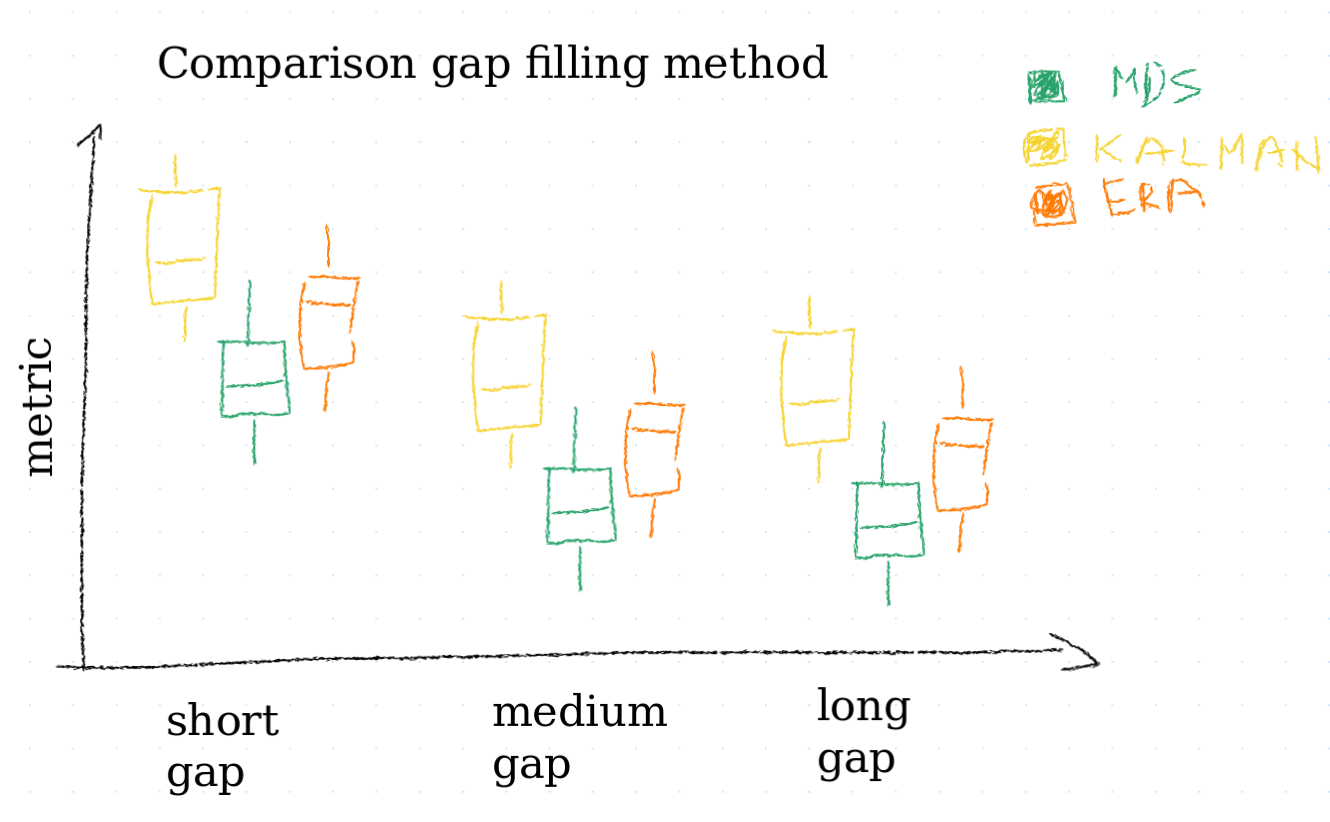
\includegraphics[width=\textwidth]{images/plot_example_comp_methods.png}

in addition:
\begin{itemize}
    \item In the Appendix make the same plot, but separate for each variable.
    \item maybe: repeat the same plot with a different metric
    \item maybe: put the results into a table
\end{itemize}

\subsection{Example Timeseries}

\textbf{goal} Show how a Kalman Filter Gap filling looks like and the uncertainty 

\begin{itemize}
    \item a few sample variables (max 3/4)
    \item a representative gap length
    \item manually choose interesting gaps (2-4)
    \item no gap in other variable
\end{itemize}

This is the most intuitive way of looking at gap filling and can select the gaps for highlighting the strengths and weakness of the filter

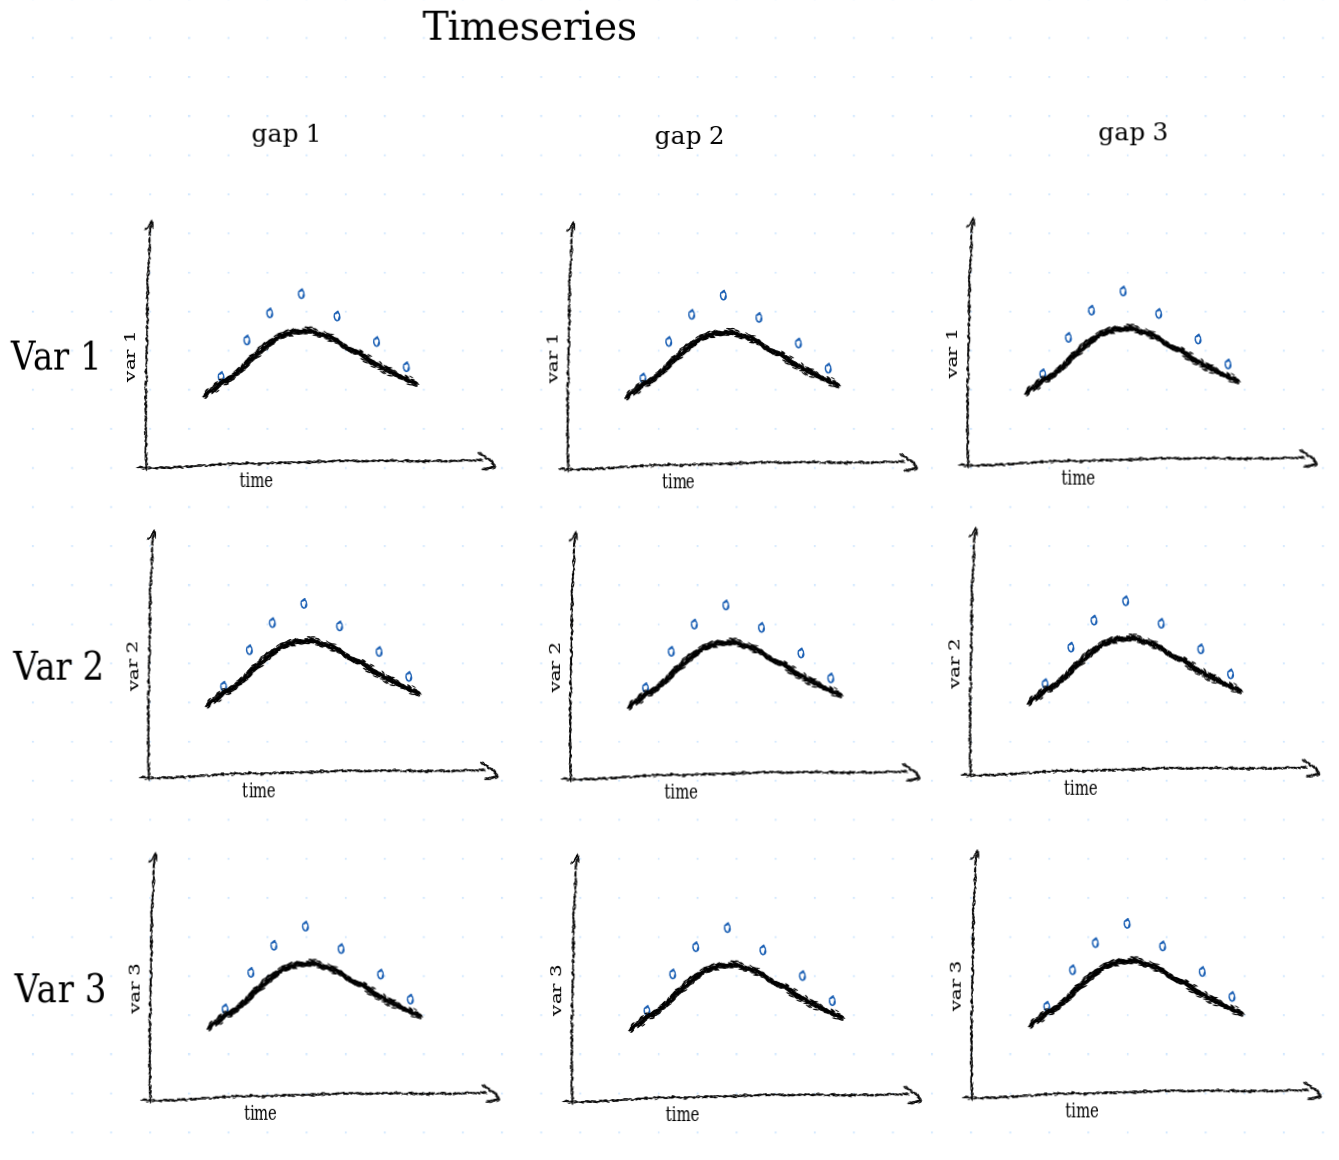
\includegraphics[width=\textwidth]{example_plot_timeseries}


\subsection{Different variables}

\paragraph{Box plot metric}

Then for every variable:
\begin{enumerate}
    \item make a random gap in the variable
    \item have all other variables without gap
    \item gap-fill
    \item compute metric
    \item repeat 1-4 for 100 times
\end{enumerate}

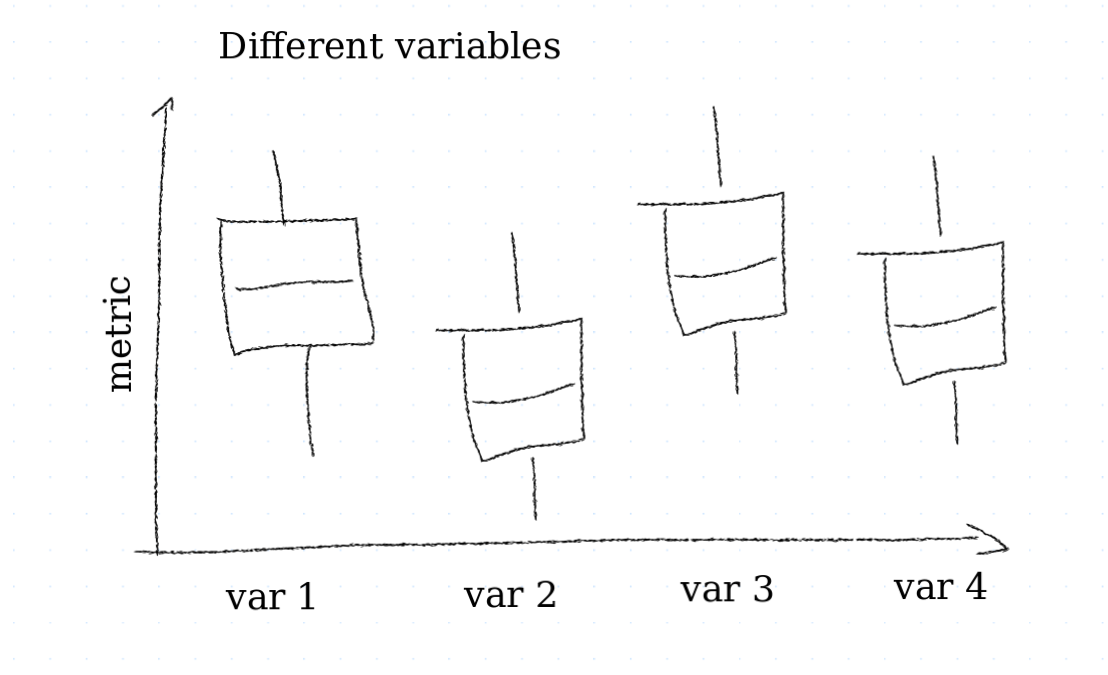
\includegraphics[width=\textwidth]{example_different_variables}


\paragraph{Maybe Table}


\begin{itemize}
    \item each variable
    \item different gap length?
    \item other variables missing
\end{itemize}

\paragraph{Maybe Scatter plot}

for each variable select representative gaps and plot predict vs actual in the gap

\subsection{Gap length}

\textbf{goal} impact of the gap length on the gap filling

select 10 different gap lengths

Then for every variable:
\begin{enumerate}
    \item make a random gap in the variable
    \item have all other variables without gap
    \item gap-fill
    \item compute metric
    \item repeat 1-4 for 100 times
\end{enumerate}

plot relation gap length / metric for all variable together

in the appendix separate variables

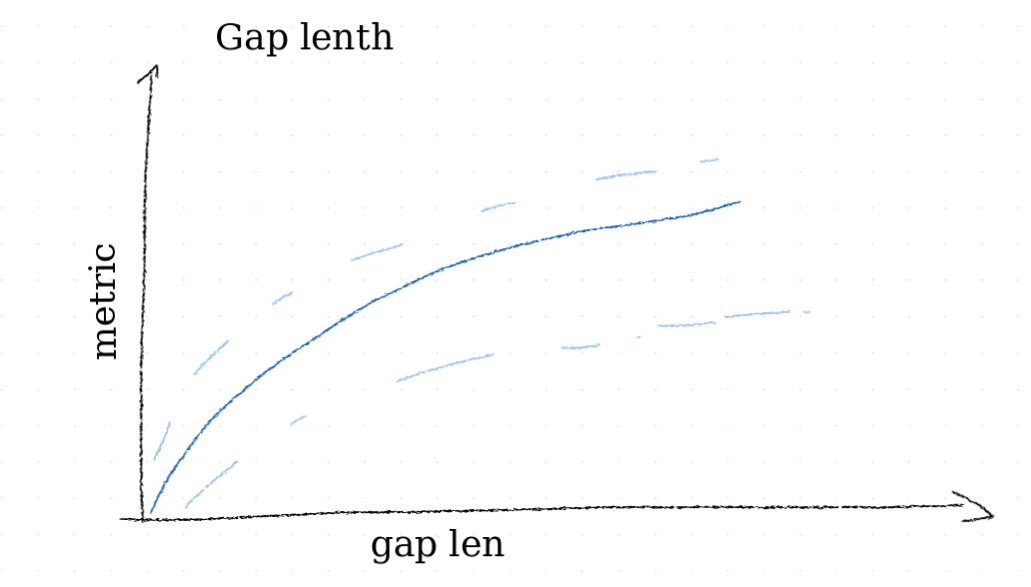
\includegraphics[width=\textwidth]{example_plot_gap_len}

\subsection{Control}

\textbf{goal} show how the use of the control (ERA-5 data) in the gap is impacting the predictions

\begin{itemize}
    \item take many gaps
    \item average metric between all variables
    \item assume that all the other variables are present
\end{itemize}

\paragraph{boxplot}

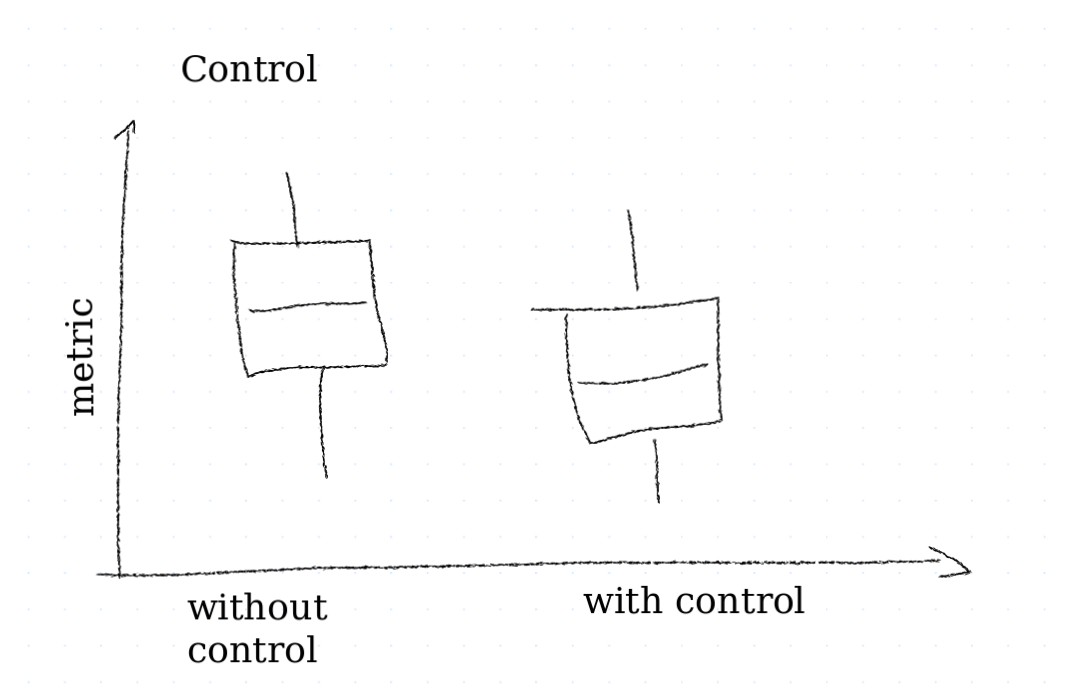
\includegraphics[width=\textwidth]{example_control}


\subsection{Other variables missing}

Goal: show how the presence/absence of other variables in the gap is impacting the predictions

- all variables
- no variables
- mean n variables present

\paragraph{boxplot}

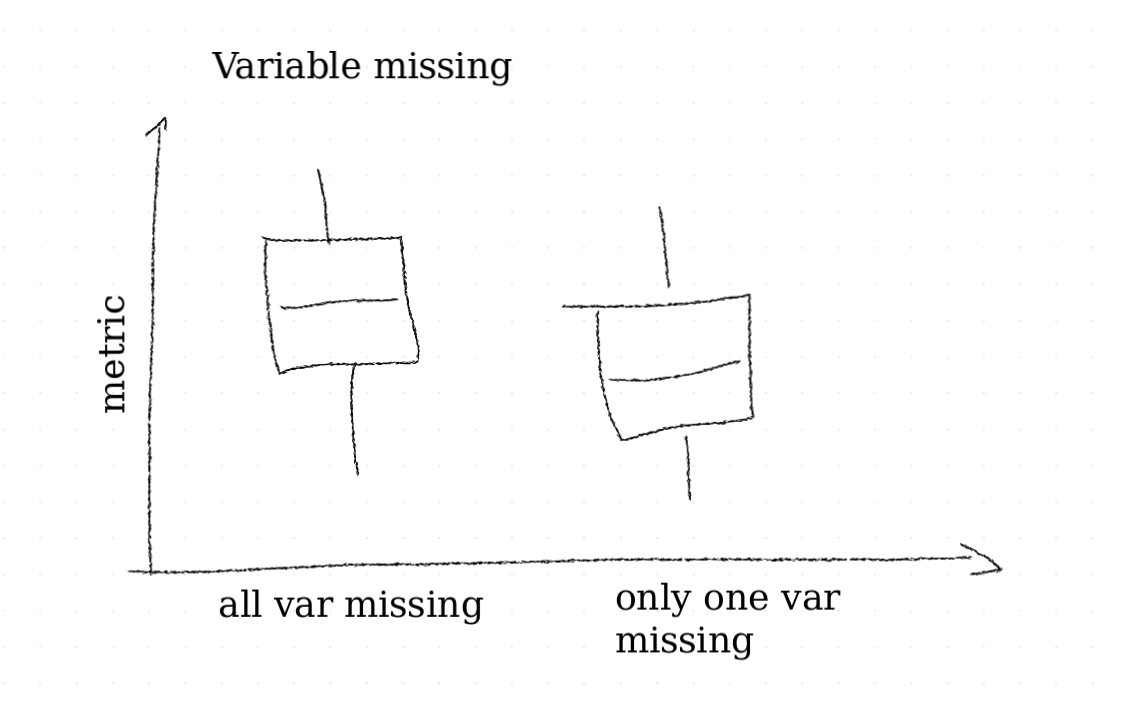
\includegraphics[width=\textwidth]{example_var_missing}




\subsection{Numerical Stability}

\begin{figure}
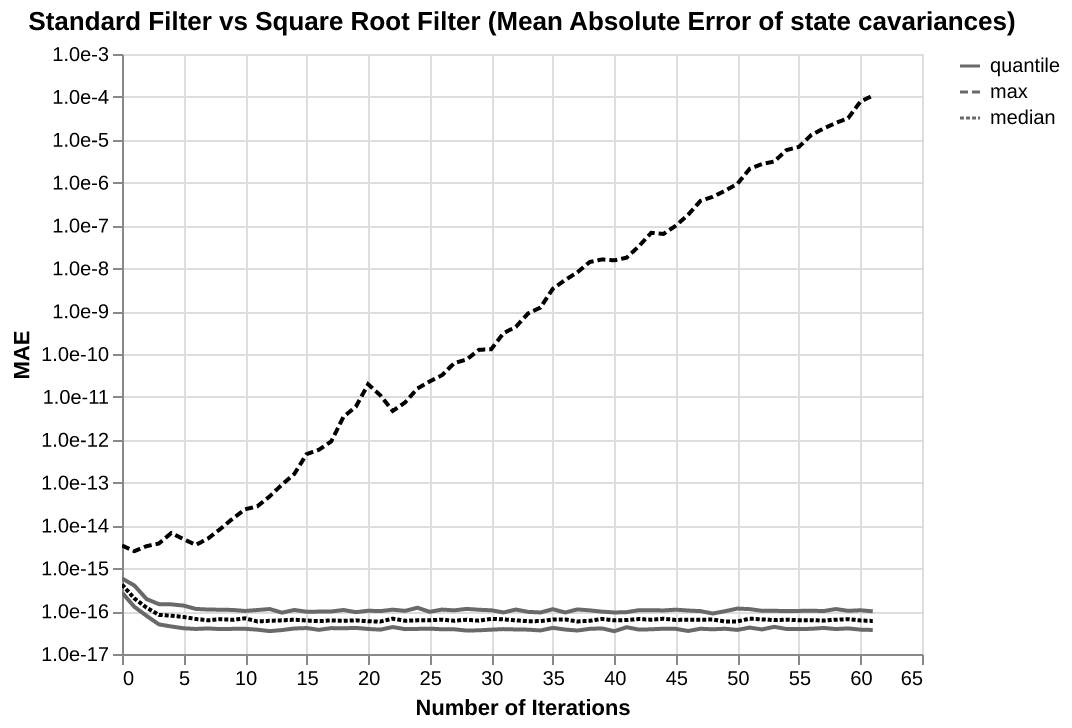
\includegraphics[width=\textwidth]{numerical_stability}
 \caption{Comparison of standard Kalman Filter implementation and Square Root Filter. For 100 times the filter has been initialized with random parameters (drawn from a uniform distribution range 0-1) and then filtered 62 observations. At each filter iteration calculated the Mean Absolute Error (MAE) between the state covariance from the standard filter and the square root filter. The plot shows the median, 1 and 3 quartile and the maximum of the MAE across the 100 samples. You can see that usually the two filter implementations agree, but for a few parameters combinations the error is growing with the number of iterations of the filter suggesting a numerical stability issue. After 62 iterations the standard filter crashes because the covariance is not positive definite anymore. The initial bigger error can be explained by the slightly different initial state covariance.}
\end{figure}



\subparagraph{}

\section{Discussion}

\subsection{Importance and use of better gap filling}


\subsubsection{Variable comparison}

difference between variables

\subsection{Limitations Kalman Filters}

\begin{itemize}
    \item assumptions of the filter
    \item long gaps
    \item shift of control variable
    \item training to different conditions
\end{itemize}

\subsection{Model deployment}

what is missing to actually use the model in production

\begin{itemize}
    \item Find optimal context before/after filter
    \item train model for different sites / fine tuning
    \item use ERA-5 Land data
\end{itemize}


\subsection{Gap filling quality assessment}

\begin{itemize}
    \item realistic gaps properties (length/other variables missing/time of day)
    \item importance of metrics
\item need to have a better analysis of gaps in fluxnet
\end{itemize}

\subsection{Improvements}

\begin{itemize}
\item NN for control! the ERA bias can change over time
\end{itemize}




\section{Conclusions}



\section*{References}

\printbibliography

\section*{Appendix}

\subsection{Proof for eigenvalues of $CC^T$}

The eigenvalues of the transpose of a matrix are the same of the eigenvalues of a matrix

The properties of the eigenvalues is that $Ax=\lambda x$ for any vector $x$

Then $CC^Tx=C(\lambda x) = \lambda Cx = \lambda^2 x$

\subsection{UD Filter}


This is not relevant anymore, keeping this for now

The UD filter (\cite{bierman_numerical_1977}) is named after the $UDU^T$ decomposition\footnote{In the literature $U$ is a lower \textbf{unit} triangular matrix, but the PyTorch routine just makes lower triangular matrices. In my understanding this makes no difference in the derivation of the equations}, which is also known as the $LDL^T$ decomposition (\cite{golub_matrix_2013}) and it always exists for a positive definite matrix. Where $U$ is a lower triangular matrix and $D$ is a diagonal matrix.

The UD Filter never computes the state covariance matrix $P$, but propagates the $U$ and $D$ components of the matrix to improve the numerical stability. Hence, the filter equations need to be rewritten by using only the $U$ and $D$ components and never the $P$ matrix

\subparagraph{Measurement update}

After each observation at time $t$ the state covariance is updated according to equation \ref{filter_correct}, which is here repeated (for notation simplicity the time subscripts are removed):

$$ P = P^- - P^-H^T(HP^-H^T + R)^{-1}HP^-$$

The goal is to obtain the $U$ and $D$ factors of $P$ given the $U^-$ and $D^-$ factors of $P^-$.

Letting:
\begin{itemize}
    \item $P = UDU^T$
    \item $P^- = U^-D^-U^{-T}$, with $U^{-T}$ being the transpose of $U^-$ not the transpose of the inverse of $U$
    \item $v = U^{-T}H^T$
\end{itemize}
then 
\begin{align}
    &UDU^T = \\
    &= U^-D^-U^{-T} - U^-D^-U^{-T}H^T\left(HU^-D^-U^{-T}H^T + R\right)^{-1}HU^-D^-U^{-T} \\
    &= U^-\left[D^- - D^-v(v^TD^-v+R)^{-1}v^TD^- \right]U^{-T}
\end{align}

If you do a UD decomposition of $\left[D^- - D^-v(v^TD^-v+R)^{-1}v^TD^- \right] = BDB^T$, where $B$ is a lower triangular matrix and $D$ is a diagonal matrix, then 

\[ UDU^T = U^-(BDB^T)U^{-T} = (U^-B)D(U^-B)^{T}) \]

$D$ is the diagonal factor of $P$ as and $U$ is equal to $U^-B$, since $U^-B$ is a lower triangular matrix as is the products of two lower triangular matrices.

Therefore, to perform the measurement update step it is necessary to compute the $UDU^T$ decomposition of $\left[D^- - D^-v(v^TD^-v+R)^{-1}v^TD^- \right]$, which can be implemented using the \verb|torch.linalg.ldl_factor| function.

\subparagraph{Time update}

The state covariance at time $t$ is obtained from the state at time $t-1$ according to the equation \ref{filter_predict}, which is here repeated:

$$ P_t = AP_{t-1}A^T + Q$$

The goal is to obtain the $U_t$ and $D_t$ factors of $P_t$ given the $U_{t-1}$ and $D_{t-1}$ factors of $P_{t-1}$.

Letting:

\begin{align}
    Q &= GD_QG^T\\
    W &= \begin{bmatrix}AU_{t-1}&G\end{bmatrix}\\
    D_w &= \begin{bmatrix}D_{t-1} & 0 \\ 0& D_Q \end{bmatrix}
\end{align}

where $D_Q$ is diagonal and $G$ is lower triangular (the UD decomposition of Q), then:

\begin{equation}
\begin{split}
   P &= WD_wW^T = \\
&=\begin{bmatrix}AU_{t-1}&G\end{bmatrix}\begin{bmatrix}D_{t-1} & 0 \\ 0& D_Q \end{bmatrix}\begin{bmatrix}U^T_{t-1}A^T\\G^T\end{bmatrix} \\
&= AU_{t-1}D_{t-1}U^T_{t-1}A^T + GD_QG^T  
\end{split}
\end{equation}

Then if we can find decompose $W$ as matrices $U_tV$ where $U_t$ is a lower triangular matrix such as that $VD_wV^T$ is a diagonal matrix then

\begin{equation}
    P_t = (U_tV)D_w(U_tV)^T = U_tD_tU_t
\end{equation}

so we have the $U_t$ and $D_t$ factors of $P_t$

This decomposition can be efficiently implemented in PyTorch using some modifications of the QR decomposition \footnote{\url{https://pytorch.org/docs/stable/generated/torch.linalg.qr.html}}

\subsubparagraph{PyTorch Implementation}

The QR decomposition in PyTorch  decompose a matrix $A = QR$, where $Q$ is an orthogonal matrix and $R$ is an upper triangular matrix.
However, for the filter there are two changes that needs to be made:
\begin{enumerate}
    \item decompose into the product of the lower triangular matrix and a diagonal matrix $A = LQ$
    \item have a weighted decomposition regarding a matrix $D$, such as that $QDQ^T = I$ instead of $QQ^T = I$
\end{enumerate}

\sssparagraph{1) Lower triangular matrix}

To obtain a lower triangular matrix from the $QR$ decomposition, you can compute the QR decomposition of $A^T=QR$ and then $A = R^TQ^T$ where $R^T$ is a lower triangular matrix and $Q^T$ is still an orthogonal matrix.

\sssparagraph{2) Weigthed decomposition}

The QR decomposition can be used to have a weighted decomposition \footnote{\url{https://scicomp.stackexchange.com/a/33436}}, where $QDQ^T = I$ instead of the $QQ^T = I$.
If $D$ is positive definite, it is possible to apply the Cholesky decomposition of $D = CC^T$. Then you can compute the QR factorization of $CA=UR$, where $U$ is an orthogonal matrix and $R$ is an upper triangular matrix. Then can define $Q=C^{-1}U$. This can be proved as 
$Q D Q^T = C^{-1}U CC^TU^T(C^{-1})^T= I$
In the filter context $D$ is a diagonal matrix computing so the Cholesky decomposition can be efficiently done by taking the square root of every element.

\sssparagraph{Summary} $W$ can be decomposed as $W=U_tV$ with the following procedure:

$$(C_{D_W}W)^T = QR$$ using \verb|torch.linalg.qr| and then defining $U_t = R^T$ and $V=C_{D_W}^{-1}Q^T$


\end{document}

